\documentclass{article}
\usepackage[
        a4paper,% other options: a3paper, a5paper, etc
        left=3cm,
        right=3cm,
        top=3cm,
        bottom=4cm,
        % use vmargin=2cm to make vertical margins equal to 2cm.
        % us  hmargin=3cm to make horizontal margins equal to 3cm.
        % use margin=3cm to make all margins  equal to 3cm.
]{geometry}
%\usepackage[utf8x]{inputenc}
\usepackage{graphicx}
\usepackage{caption}
\usepackage{enumerate}
\usepackage{subcaption}
\usepackage[procnames]{listings}
\usepackage{color}
\usepackage{amssymb}
\usepackage{amsmath}      
\usepackage{comment}
\usepackage{hyperref}
\usepackage{blindtext}
\usepackage[scaled=.8]{sourcecodepro}
\setcounter{section}{+1}
\definecolor{codegreen}{rgb}{0,0.6,0}
\definecolor{codegray}{rgb}{0.5,0.5,0.5}
\definecolor{codepurple}{rgb}{0.58,0,0.82}
\definecolor{backcolour}{rgb}{0.95,0.95,0.92}
 
%\renewcommand*\ttdefault{pcr} 
 
\lstdefinestyle{mystyle}{
    backgroundcolor=\color{backcolour},   
    commentstyle=\color{codegreen},
    keywordstyle=\color{blue},
    numberstyle=\tiny\color{codegray},
    stringstyle=\color{codepurple},
    basicstyle=\ttfamily,
    breakatwhitespace=false,         
    breaklines=true,                 
    captionpos=b,                    
    keepspaces=true,                 
    numbers=left,                    
    numbersep=5pt,                  
    showspaces=false,                
    showstringspaces=false,
    showtabs=false,                  
    tabsize=2
}

\title{Lab Assignment 4\\ {\Large Convolutional Neural Networks}}
\date{\today}
\author{
 	Eleftherios Karamoulas - S3261859\\ 
	Panagiotis Tzafos - S3302148\\
}

\lstset{style=mystyle, language=Matlab}
\begin{document}
\maketitle
\section{Theory questions}
\begin{enumerate}
\item The pooling layer serves to progressively reduce the spatial size of the representation, to reduce the number of parameters and amount of computation in the network, and hence to also control overfitting(CS231n lecture). In practice, its use is to downsample its input, reducing the amount of resources that the network needs in order to perform the computations by reducing the dimensions of the input using a filter, a stride and an elementwise activation function. Also, after the downsampling it is obvious that the network will have less parameters. As a result, it will be able to generalize better in new situations and avoid overfitting(small training set error, large error for new examples). 
\item
Weight sharing is a very important feature, as it can dramatically reduce the number of weights(less computations). The idea behind this is that the number of unique sets of weights can be equal to the depth dimension size. This can applied because of the fact that, assuming that a single depth slice weight configuration is associated with a single feature that our network is looking for(edges, circles etc.), in every single one spatial region that the filter checks, it responsible of tracing these specific features. \textcolor{red}{???(filters depth not sure equal)}
\item
\item
\begin{enumerate}
\item From the given data and the formula to compute the output we have that W=12, F=3, P=0 and S=1, so output = W - F + 2 * P / S + 1 = 12 - 3 + 2 * 0 / 1 + 1 =  10 and because we have 3 filters the total neurons will be 10 x 10 x 3 = 300.\\
\item
 The input layer is our image and if we assume that  each pixel is one neuron our input layer consists of 12 x 12 = 144 neurons and each of them will be fully connected to our neurons in the hidden layer which consists of 300 neuros. As a result the total connections between input and hidden layer will be 144 x 300 = 43200.\\
\textcolor{red}{Complete subquestion about parameters}
\end{enumerate}
\item This approach to solve the car decision problem is questionable because even though we can use CNN's and get a network that can decide between cars an average solution, the features that characterise the car can be subjective for different customers depending on their needs and comforts.
\end{enumerate}
\setcounter{section}{+3}
\section{Convolutional Layer}
\lstinputlisting[caption={cnnConvolve.m},label={code:bar}]{cnn/cnnConvolve.m}
\section{Mean Pooling Layer}
\lstinputlisting[caption={cnnPool.m},label={code:bar}]{cnn/cnnPool.m}
\section{Forward Pass}
\lstinputlisting[caption={cnnCost.m},label={code:bar}]{cnn/cnnCost.m}
\section{Experiments}
\begin{enumerate}
\item \textcolor{red}{Question 1}
\item In the beginning of the training we see that our filters look like random noise patches but as our training progresses we see that the filters achieve more structure and finally after 3 epochs we can see clearly on them shapes e.g.(lines, angles, curves) that they can recognize on images that we feed to our network.
\begin{figure}[!h]
    \centering
    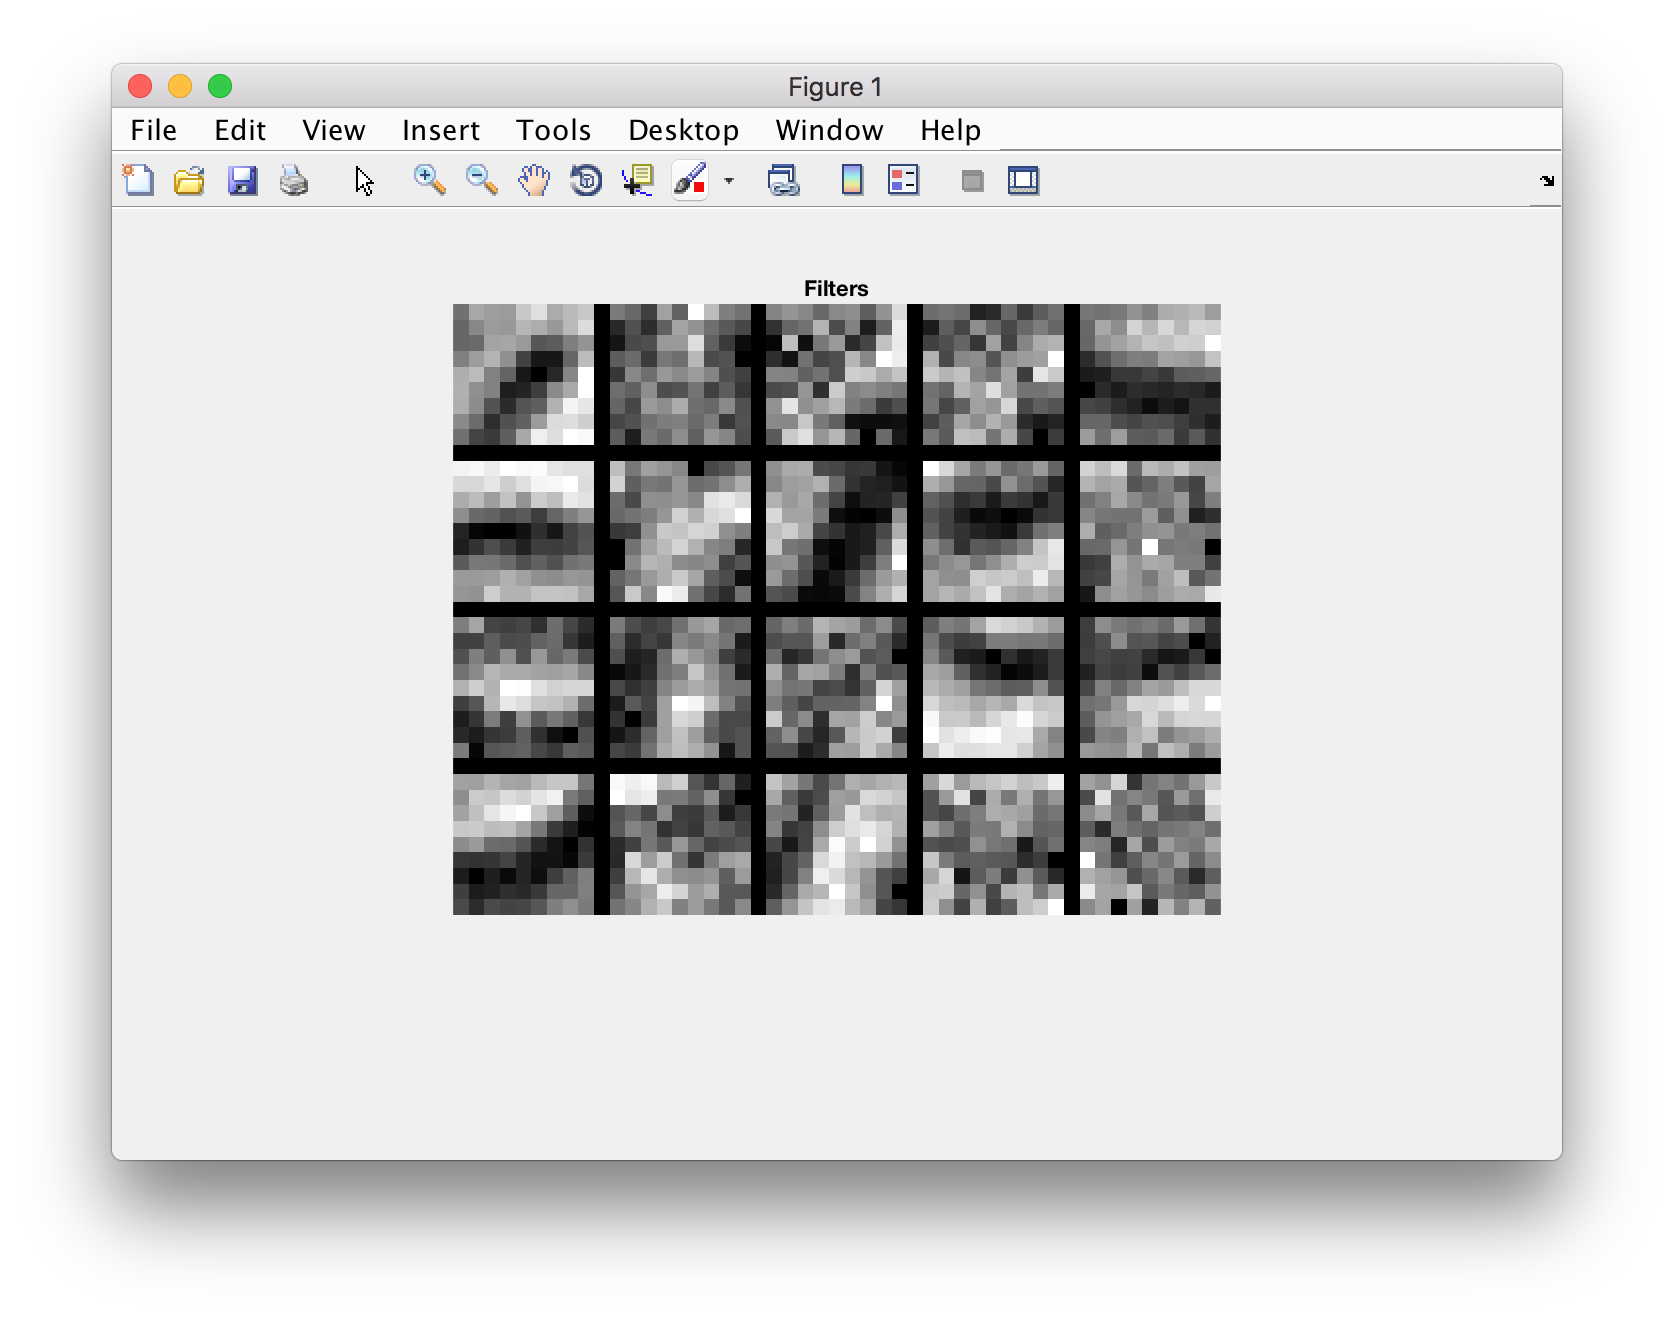
\includegraphics[width=1\textwidth]{filters.png}
    \caption{Filters after 3 epochs}
    \label{fig:picture}
  \end{figure}
\item Our network accuracy after 3 epochs is 97.24\%
\end{enumerate}
\end{document}
